\documentclass[12pt,a4paper,UTF8]{article}
\usepackage{ctex} % Chinese support
\usepackage{graphicx} % Insert images
\usepackage{subfigure}
\usepackage{float}
\usepackage{listings} % Print source code
\usepackage{color} % Color support
\usepackage{booktabs} % Professional table support
\usepackage{pdflscape} % Landscape pages support in PDF
\usepackage{hyperref} % Hypertext links support for cross-referencing
\usepackage{amsmath,mathtools}
\usepackage{ulem} % strikethrough

% Customize hyperref format (it's set to no special format here)
\hypersetup{hidelinks}

% Declare directories to search for graphics files for graphicx
\graphicspath{{figures/}}

% Define source code style for listings
\lstdefinestyle{verilog-style}{
	language=Verilog,
	basicstyle=\ttfamily\footnotesize,
	keywordstyle=\bfseries\color[rgb]{0, 0, 1},
	identifierstyle=\color[rgb]{0.5, 0.3, 0.1},
	stringstyle=\color[rgb]{0.6, 0.1, 0.1},
	commentstyle=\itshape\color[rgb]{0.05, 0.5, 0.05},
	backgroundcolor=\color[gray]{0.95},
	numbers=left,
	numbersep=5pt,
	numberstyle=\color[gray]{0.6},
	breaklines=true,
  escapeinside={(:}{:)}
}

\newcommand{\reporttitle}[2]{
  \LARGE\textsf{#1}\quad\underline{\makebox[12em]{#2}}
}

\newcommand{\reportinfo}[2]{
  \large\makebox[5em]{\textsf{#1}}\quad\underline{\makebox[18em]{#2}}
}

\begin{document}
\begin{titlepage}
  \centering
  \vspace*{\fill}
  {\Huge\textsf{数字电路与数字系统实验}} \\ [100pt]
  \reportinfo{实验名称}{exp12 简单计算机系统} \\ [10pt]
  \reportinfo{院系}{计算机科学与技术系} \\ [10pt]
  \reportinfo{姓名及学号}{} \\ [10pt]
  \reportinfo{}{} \\ [10pt]
  \reportinfo{班级}{数字电路与数字系统实验1班} \\ [10pt]
  \reportinfo{邮箱}{} \\ [10pt]
  \reportinfo{}{} \\ [10pt]
  \reportinfo{实验时间}{2020 年 12 月 19 日} \\ [10pt]
  \vspace*{\fill}
\end{titlepage}
\tableofcontents
\newpage


\part{准备工作}
\section{实验目的}
\begin{itemize}
  \item 学习计算机系统的组成和架构
  \item 学习设计更大型的Verilog工程
  \item 学习MIPS汇编指令
  \item 自己动手搭建一个CPU
  \item 学习编写一些汇编指令,使其能在自己编写的CPU上运行
\end{itemize}


\section{实验原理}
\begin{description}
  \item[CPU处理的六个阶段] 取指、译码、执行、访存、写回、更新PC。
  \item[MIPS指令解码的原理] MIPS指令分为三种基本类型:R-Type、I-Type、
        J-Type,需要根据不同的类型采用不同的解码方式。
  \item[内存的设计] 内存需要划分一块区域作为显存,显示器根据显存的内容
        把对应的字符输出到显示屏上。因为键盘按键需要回显、CPU执行的指令中
        包含读写内存的指令,所以会有不同的模块会对内存进行读写,需要设计好
        控制信号,根据时序进行内存读写。
\end{description}
\begin{figure}[H]
  \centering
  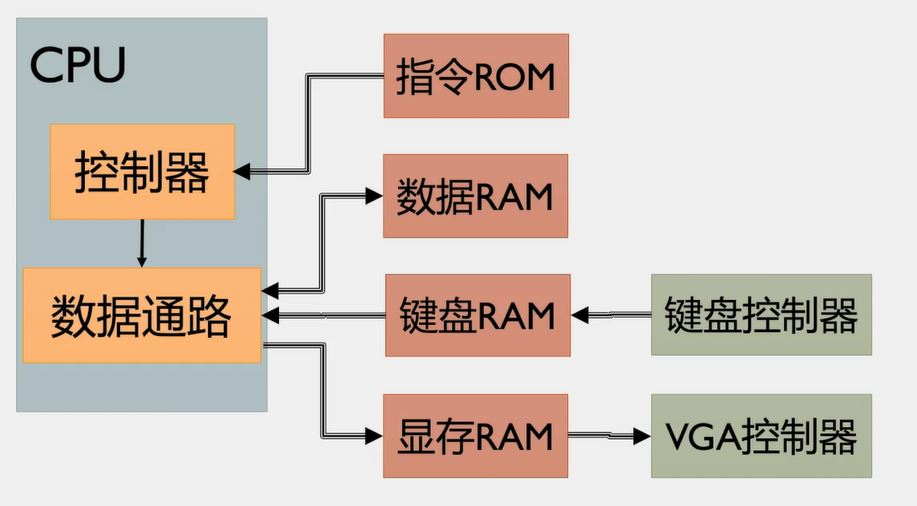
\includegraphics[width=0.8\textwidth]{system_struct.JPG}
  \caption{计算机系统架构}
  \label{system_struct}
\end{figure}


\section{实验环境/器材}
\begin{itemize}
  \item Quartus编辑器和DE10-Standard开发平台
  \item FPGA开发板
  \item 带有PS/2接口的键盘
  \item 带有VGA接口的显示器
\end{itemize}
\newpage

\part{实验过程}
\section{存储器部分}
需要构建的存储器有:指令存储器,寄存器存储器,
以及内存(划分成显存区和数据区)存储器。

寄存器存储器的元素大小为32位,指令存储器和
内存存储器的元素大小为8位。

这些存储器都是用RAM实现的。它们有一些相同的接口:

\begin{description}
  \item[输入:]
  \item[clk] 时钟信号
  \item[clrn] 清零信号(低有效)
  \item[re] 读使能信号
  \item[read\_addr] 读地址
  \item[we] 写使能信号
  \item[write\_addr] 写地址
  \item[write\_data] 写数据
  \item[输出:]
  \item[read\_data] 读数据
  \item[read\_finished] 读数据完毕的信号
  \item[write\_finished] 写数据完毕的信号
\end{description}

读和写的过程是这样进行的:
\begin{lstlisting}[style=verilog-style]
always @ (negedge clk) begin // read
  if (clrn == 0 || (re == 0)) begin
    read_finished <= 0;
  end else begin
    if (re) read_data <= ram[read_addr];
    read_finished <= 1;
  end
end

always @(posedge clk) begin // write
  if (clrn == 0 || we == 0) begin
    write_finished <= 0;
  end else begin
    ram[write_addr] <= write_data;
    write_finished <= 1;
  end
end
\end{lstlisting}

对于每个存储器的详细实现,我们会在后面相关的模块中具体介绍。
我们在这里先简单描述了一些CPU要用的接口,以便下文对CPU模块的介绍。


\section{CPU部分}
\subsection{CPU与三个存储器}
前面所描述的三个存储器中,只有寄存器存储器是完全归CPU控制、不需要
被其他模块访问的,所以寄存器存储器可以作为CPU的子模块。
但是它有个特殊的地方,就是它有两个读接口。因为MIPS汇编中有3操作数
的指令,所以它要同时读两个寄存器,然后把结果写到第三个寄存器里。
因此寄存器模块中的读操作代码变成了这样:
\begin{lstlisting}[style=verilog-style]
always @ (negedge clk) begin // read
  if (clrn == 0 || (re1 == 0 && re2 == 0)) begin
      read_finished <= 0;
  end else begin
      if (re1) read_data1 <= regs[read_addr1];
      if (re2) read_data2 <= regs[read_addr2];
      read_finished <= 1;
  end
end
\end{lstlisting}

对于另外两个存储器,即指令存储器和内存,它们需要放在CPU外部,
也就是顶层模块之下。这两个存储器和CPU交互的信号需要通过顶层模块
来进行传递,所以CPU模块会有很多与它们交互的接口。

\begin{figure}[H]
  \centering
  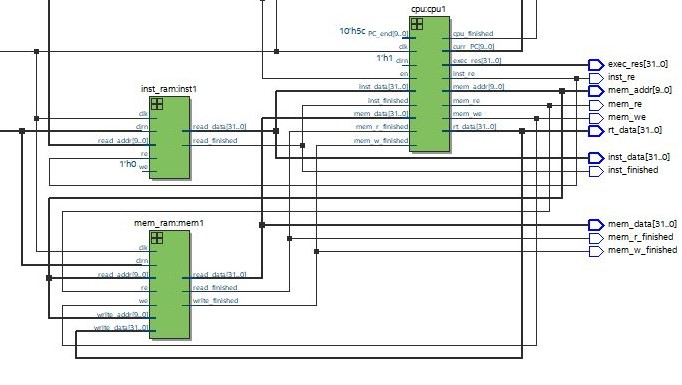
\includegraphics[width=1\textwidth]{cpu_module.jpg}
  \caption{CPU模块的部分RTL视图}
  \label{cpu_module}
\end{figure}

\subsection{处理指令之前的准备}
除了与存储器交互的输入输出接口之外,CPU模块还需要这些接口:

\begin{description}
  \item[输入:]  \hspace*{\fill}
  \item[en] 使能信号
  \item[clk] 时钟信号
  \item[clrn] 清零信号(低有效)
  \item[PC\_end] 指令存储器的末尾(最后一条指令的PC再加4)
  \item[输出:]
  \item[cpu\_finished] 所有指令执行完毕
\end{description}

我们是按状态机的方式实现CPU的。CPU处理经过的六个阶段就是我们
要设计的六个状态。我们用变量state表示当前CPU所处的状态,用一个
case语句根据state的值进行选择,从而处理当前阶段的任务。state为0时
表示CPU启动,state从1到6分别对应取指、译码、执行、访存、写回、更新PC。

\begin{lstlisting}[style=verilog-style]
always @ (posedge clk) begin
  if (clrn == 0 || en == 0) begin
    state <= 0;
    curr_PC <= 0;
  end else begin
    inst_re <= 0;
    reg_re1 <= 0;
    reg_re2 <= 0;
    reg_we <= 0;
    mem_re <= 0;
    mem_we <= 0;
    R_en <= 0;
    I_en <= 0;

    case(state)
      0: begin
        curr_PC <= 0;
        next_PC <= 0;            
        state <= 1;
      end
      /* (:省略了一些case:) */
    endcase
end
\end{lstlisting}


\subsection{处理指令的六个阶段}
\subsubsection{取指(instruction fetch)}
\begin{description}
  \item[要处理的工作:] \hspace*{\fill}
        \begin{enumerate}
          \item 根据PC值到指令存储器中取出32位指令码inst\_data。
          \item next\_PC = curr\_PC+4。
          \item state置为2。
        \end{enumerate}
  \item[涉及到的模块:] inst\_ram(指令存储器)
\end{description}

\begin{lstlisting}[style=verilog-style]
case(state)
  /* (:部分case已省略:) */
  1: begin // instruction fetch
    inst_re <= 1;
    next_PC <= curr_PC + 4;
    if (inst_finished) state <= 2;
  end
endcase
\end{lstlisting}


\subsubsection{译码(decode)}
\begin{description}
  \item[要处理的工作:] \hspace*{\fill}
        \begin{itemize}
          \item assign赋值:op, rs\_addr, rt\_addr, rd\_addr,
                shamt, funct, imm16, tar。
          \item 从寄存器存储器中根据寄存器地址(rs\_addr, rt\_addr)
                取出寄存器操作数(rs\_data, rt\_data)。
          \item 根据opcode判断指令类型。如果是 J\_TYPE,
                则设置next\_PC,然后state转至`更新PC'阶段。
                否则,设置指令类型标志inst\_type (R\_TYPE, I\_TYPE)。
          \item 完成之后state置3。
        \end{itemize}
  \item[涉及到的模块:] reg\_ram(寄存器存储器)
\end{description}

\begin{lstlisting}[style=verilog-style]
case(state)
  /* (:部分case已省略:) */
  2: begin // decode
    reg_re1 <= 1;
    reg_re2 <= 1;
    if (reg_r_finished) begin
      state <= 3;
      if (op == 6'h2) begin // J_TYPE
          next_PC <= {4'b0, tar, 2'b0}; // [`INST_RAM_WIDTH-1:0]
          state <= 6;
      end else if (op == 6'h0) begin  // R_TYPE
          inst_type <= `R_TYPE;
          reg_w_addr <= rd_addr;
      end else begin
          inst_type <= `I_TYPE;
          reg_w_addr <= rt_addr;
      end
    end
  end
endcase
\end{lstlisting}


\subsubsection{执行(execute)}
\begin{description}
  \item[要处理的工作:] \hspace*{\fill}
        \begin{itemize}
          \item 根据指令类型inst\_type (R\_TYPE, I\_TYPE),
                设置相应的使能R\_en, I\_en。
          \item 根据操作数进行运算,得到运算结果exec\_res
                及其目标类型dst\_type。
          \item 对于计算结果的目标类型(dst\_type),定义宏如下:
                \begin{description}
                  \item[DST\_RD] 计算结果直接存入rd寄存器
                  \item[DST\_RT] 计算结果直接存入rt存储器
                  \item[DST\_MEM\_L] 访存后存入rt存储器
                  \item[DST\_MEM\_S] 将rt存储器中的值写入内存
                  \item[DST\_PC] 赋值给next\_PC
                \end{description}
          \item 根据finished\_R或finished\_I信号更新state。
                当dst\_type为DST\_MEM\_L\linebreak[4]
                或DST\_MEM\_S时,state更新为4;
                当dst\_type为DST\_PC时,state更新为6;
                否则state更新为5。
        \end{itemize}
  \item[涉及到的模块:] \hspace*{\fill}
        \begin{enumerate}
          \item R\_exec
                \begin{description}
                  \item[输入:] \hspace*{\fill}
                  \item[clk] 时钟信号
                  \item[clrn] 清零信号(低有效)
                  \item[R\_en] 使能信号
                  \item[op, rs\_data, rt\_data, shamt, funct] \hspace*{\fill}
                  \item[输出:] \hspace*{\fill}
                  \item[res\_R] 计算结果
                  \item[dst\_type\_R] 计算结果的目标类型\\
                        此模块中该参数统一输出为DST\_RD
                  \item[finished\_R] 当前阶段已经处理完成,
                        可以进行下一阶段(更新state)
                \end{description}
          \item I\_exec
                \begin{description}
                  \item[输入:] \hspace*{\fill}
                  \item[clk] 时钟信号
                  \item[clrn] 清零信号(低有效)
                  \item[I\_en] 使能信号
                  \item[op, rs\_data, imm16] \hspace*{\fill}
                  \item[输出:] \hspace*{\fill}
                  \item[res\_I] 计算结果
                  \item[dst\_type\_I] 计算结果的目标类型\\
                        对于此模块中的该参数,除了branch指令
                        输出为DST\_PC、指令lw和sw输出分别为
                        DST\_MEM\_L和DST\_MEM\_S外,
                        其余指令统一输出为DST\_RT
                  \item[finished\_I] 当前阶段已经处理完成,
                        可以进行下一阶段(更新state)
                \end{description}
        \end{enumerate}
\end{description}

\begin{lstlisting}[style=verilog-style]
case(state)
  /* (:部分case已省略:) */
  3: begin // execute
  if (inst_type == `R_TYPE) begin
      R_en <= 1;
      if (finished_R) begin
        exec_res <= res_R;
        dst_type <= dst_type_R;
        state <= 5;
      end
  end else if (inst_type == `I_TYPE) begin
      I_en <= 1;
      if (finished_I) begin
        dst_type <= dst_type_I;
        if (dst_type_I == `DST_MEM_L
        || dst_type_I == `DST_MEM_S) begin
            mem_addr <= res_I[`MEM_RAM_WIDTH-1:0];
            state <= 4;
        end else if (dst_type_I == `DST_PC) begin
            if (res_I) next_PC <= {14'b0, imm16, 2'b0} + curr_PC + 4;
            state <= 6;
        end else begin
            exec_res <= res_I;
            state <= 5;
        end
      end
  end
  end
endcase
\end{lstlisting}


\subsubsection{访存(memory)}
\begin{description}
  \item[要处理的工作:] \hspace*{\fill}
        \begin{itemize}
          \item 根据dst\_type设置内存的读使能或写使能。
          \item 完成之后state置5(DST\_MEM\_L)或6(DST\_MEM\_S)。
        \end{itemize}
  \item[涉及到的模块:] mem\_ram(寄存器存储器)
\end{description}

\begin{lstlisting}[style=verilog-style]
case(state)
  /* (:部分case已省略:) */
  4: begin // memory
  if (dst_type == `DST_MEM_L) begin
     mem_re <= 1;
     if (mem_r_finished) begin
        exec_res <= mem_data;
        state <= 5;
     end
  end else if (dst_type == `DST_MEM_S) begin
     mem_we <= 1;
     if (mem_w_finished) begin
        state <= 6;
     end
  end
  end
endcase
\end{lstlisting}

\subsubsection{写回(write back)}
\begin{description}
  \item[要处理的工作:] \hspace*{\fill}
        \begin{itemize}
          \item 设置写使能,把计算结果回写到寄存器中。
          \item 完成之后state置6。
        \end{itemize}
  \item[涉及到的模块:] reg\_ram(寄存器存储器)
\end{description}

\begin{lstlisting}[style=verilog-style]
case(state)
  /* (:部分case已省略:) */
  5: begin // write back
    reg_we <= 1;
    if (reg_w_finished) state <= 6;
  end
endcase
\end{lstlisting}


\subsubsection{更新PC(PC update)}
\begin{description}
  \item[要处理的工作:] \hspace*{\fill}
        \begin{itemize}
          \item 设置下一个PC值(next\_PC)为下一个指令码的地址。
          \item 完成之后,如果next\_PC == PC\_end,
                那么state置0。否则说明\linebreak[4]
                next\_PC处有可执行的指令,state置1。
        \end{itemize}
\end{description}

\begin{lstlisting}[style=verilog-style]
case(state)
  /* (:部分case已省略:) */
  6: begin // PC update
    if (next_PC == PC_end) begin
      state <= 0;
    end else begin
      curr_PC <= next_PC;
      state <= 1;
    end
  end
endcase
\end{lstlisting}

\subsection{有关信号en和信号finished的时序分析}
前面有很多地方都会用到两个信号:en和finished。信号en是使能信号,
只有在它有效时,才会执行相关的处理过程。信号finished是相关过程
执行结束的标志,它只在执行完成时的那一个周期内有效。一个周期后恢复为0。
我们以读写存储器为例,分析时序如下图:
\begin{figure}[H]
  \centering
  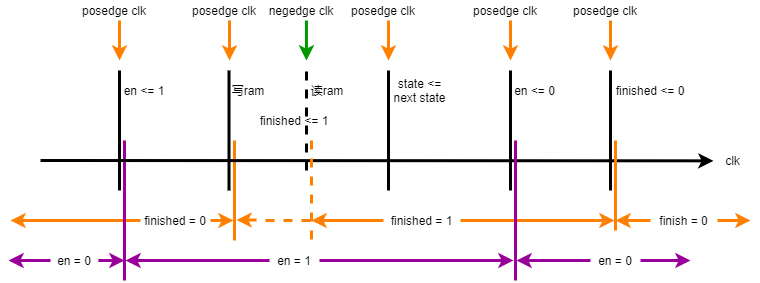
\includegraphics[width=1\textwidth]{ram_timing.png}
  \caption{读写存储器的时序分析}
  \label{ram_timing}
\end{figure}

唯一与众不同的是CPU的finished信号,它在CPU不处理指令时一直是1,
在CPU处理指令时一直为0。我们一开始对它的设置是当state为0时,
将它置为1。分析时序如下:
\begin{figure}[H]
  \centering
  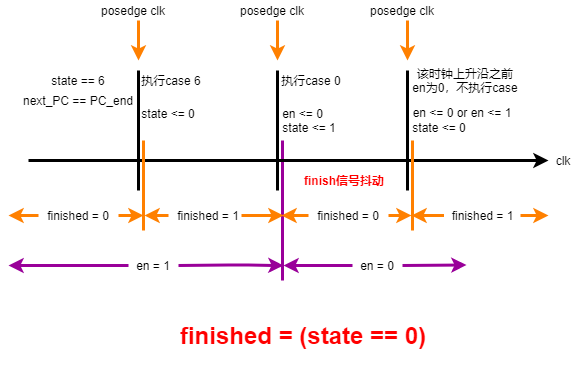
\includegraphics[width=1\textwidth]{cpu_finished_jitter.png}
  \caption{会产生抖动的cpu\_finished信号}
  \label{jitter}
\end{figure}

从图中我们可以得知,CPU在执行case6时,state被置为0,相应的
cpu\_finished信号也会随之变为1。下一个周期时,上层模块会根据
cpu\_finished信号有效而关闭CPU的使能信号,同时CPU模块在此周期
会执行case0的代码,把state置为1。这时候cpu\_finished信号也会
立即跟着变为1。再下一个周期时,此时CPU的使能信号已经被置为0了,
所以CPU不会执行case语句,而是会把state置为0并保持不变。从这开始,
在下一次CPU处理程序之前,state就一直保持为0了,cpu\_finished信号
也就一直保持为1。

所以我们发现,在CPU处理完一个程序之后、cpu\_finished信号
稳定为1之前,cpu\_finished信号会产生一个抖动。这可能会成为
某个隐患,所以我们要进行消抖。

消抖的办法有很多,我们采用的是这种方法:
\begin{figure}[H]
  \centering
  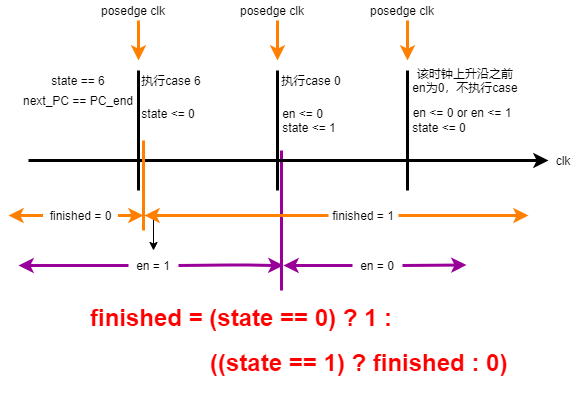
\includegraphics[width=1\textwidth]{cpu_finished_debounce.png}
  \caption{cpu\_finished信号消抖}
  \label{debounce}
\end{figure}

我们注意到cpu\_finished信号抖动是由state由0变为1引起的。所以我们
针对state为1的情况加以判断,从而避免抖动的情况。

无论消抖与否,cpu\_finished信号还有一个要做细微处理的地方。
在我们的设计中,CPU的上层模块会根据cpu\_finished信号的产生
而关闭CPU的使能信号。但是在CPU刚刚被使能的时候,state还是
保持为0的状态,如果我们此时直接根据cpu\_finished信号
把信号关闭,那么CPU就根本不会开始执行汇编指令。所以我们
需要设计好这里的时序问题,仔细思考何时才能根据cpu\_finished信号
关闭使能。处理这个细节的方法非常多,包括延长回车信号的持续时间
(我们把回车信号作为启动CPU使能信号的信号)、合理安排
if-else的顺序等等。我们采用的是一种更为保险的方法,
即在CPU启动之后隔几个周期,再去判断是否关闭CPU使能:
\begin{lstlisting}[style=verilog-style]
parameter [2:0] set_time = 5;
if (enter_flag==1) begin
  cpu_en <= 1;
  cnt <= 0;
end else if (cnt == set_time) begin
  if (cpu_finished==1) cpu_en <= 0;
end else begin
  cnt <= cnt + 1;
end
\end{lstlisting}


\subsection{CPU部分的模块结构示意图}
\begin{figure}[H]
  \centering
  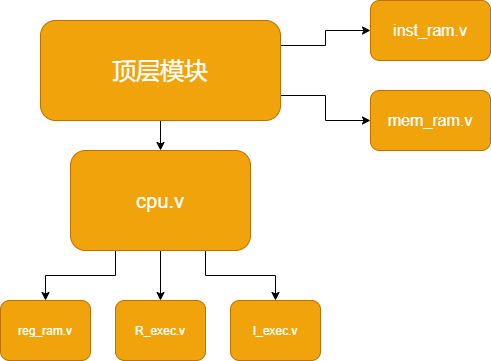
\includegraphics[width=0.8\textwidth]{cpu_struct.png}
  \caption{CPU部分的模块层次结构}
  \label{cpu_struct}
\end{figure}


\section{键盘部分}
键盘部分对比前序基础实验做了较多改动与添加,主要是保证时序一致性问题。
\begin{itemize}
  \item 在按键模块\mbox{keyboard.v}将时序同步为CLOCK\_50,
        由key\_off控制按键间隔。增加了信号func\_char,根据
        回车、退格和字符输入这些不同的情况对它进行设置。
  \item 主要添加了判断模块\mbox{check.v},用于进行字符串的匹配比较
        和给出光标的移动情况。输出的信号有:字符串判断结果prog\_type、
        针对fib和led这些软件可能存在的参数argu、
        光标移动结果cursor\_x、cursor\_y等。
        \begin{itemize}
          \item 字符串比较是通过设置尾指针的方式,使其指向一块
                缓存buf。每次回车后对缓存中的值进行比较,并输出结果。
                输出结果后缓存和尾指针都被清零。
          \item 根据按键给出的信号one\_char\_flag与回车信号prog\_change,
                设置回车命令提示信号enter\_flag。该信号在按下回车后的
                5个周期内置1,其他情况下置0。顶层模块会根据该信号
                来设置CPU的使能信号。
          \item 关于光标移动问题:引入信号cursor\_move\_en与信号
                move\_over,使其相互配合,在CLOCK\_50的时序下保持一致性。
          \item 另外,由于在计算机系统的实现原理中,内存是一个单独的模块,
                显存是内存的一部分,所以对显存的赋值操作(即按键回显)
                需要在内存模块进行。相对应的,在键盘模块中,
                键盘输出的光标位置实际上被转换成要写入的显存地址。
                我们需要实现的是把键盘输入的字符写入显存的该地址,
                然后光标移动到下一个位置。

                如果显存和光标放在同一个模块的话,写显存和移动光标就可以
                在同一个always块中进行,就像实验11那样。
                但是本实验中,写显存是在内存模块进行的,
                移动光标是在键盘模块进行的。把原本在同一always块中
                进行的操作分开放在两个always块中,如果所用的时钟信号
                频率不同,那么就会引发时序问题。

                在我们原来的实现中,光标移动部分的时钟会比CLOCK\_50慢一些,
                所以该时钟的相邻两个上升沿之间会有很多个CLOCK\_50的
                上升沿。这导致在光标移动到下一个位置之后、move\_over信号
                有效之前,这中间有很多个CLOCK\_50的上升沿。又因为设置
                显存写使能所在的always块的时钟也是CLOCK\_50,所以一旦\linebreak[4]
                one\_char\_flag信号在这期间有效,显存写使能就会以
                CLOCK\_50为周期交替置1和置0(we与write\_finished
                交互的结果)。这样一来,新的光标位置上
                就会被写入上一个按键的字符,并且光标不会继续向前移动。
                在显示器上表现出的情况为:光标移动后位置被写入了多余的量。
        \end{itemize}
\end{itemize}
键盘这边信号错综复杂,bug也频频发生。最终修改下的几个主要控制信号代码解释如下:
\subsection{we \& cursor\_move\_en \& move\_over}
\begin{lstlisting}[style=verilog-style]
always @ (posedge clk) begin
  if(clrn==0) begin
    we<=0;
    cursor_move_en<=0;
  end else begin
    if ((one_char_flag==1||we==1) && move_over==0) begin			
      if (write_finished==1) begin
        cursor_move_en<=1;
        we<=0;
      end else
        we<=1;
    end else begin
      we<=0;
      cursor_move_en<=0;
    end
  end
end

always @ (posedge clk) begin	//cursor move part
  ...      
  if(one_char_flag==0)move_over<=0;
    ...
  if(cursor_move_en==1)begin
    ...
    move_over<=1;
  end
  ...
end
\end{lstlisting}

one\_char\_flag是按键有效信号;we是显存写使能;
write\_finished是写完之后内存提供的写结束提示。

当按键有效时we置为1,显存开始写入。当写入结束时write\_finished被置为1
(write\_finished本身和写入同步时序,所以会在下一个时钟周期得到,
即write\_finished慢一个时钟沿)。
当写结束时cursor\_move\_en置1,表示光标可以移动到下一个坐标。
同时we置为0,确保这个坐标不会被写入其他值。
当光标移动完毕时,将move\_over置为1,确保we和cursor\_move\_en一直保持0。
直到按键消失说明本次按键过程全部结束,move\_over归为0。
在没有新按键的情况下,we和cursor\_move\_en仍然保持0。

\subsection{enter\_flag}
\begin{lstlisting}[style=verilog-style]
always @ (posedge clk) begin
  if(clrn==0)begin
    enter_flag<=0;
    enter_cnt<=0;
  end else begin
    if(enter_cnt==set_time) begin
      enter_flag<=0;
    end else if(prog_change==1) begin
      enter_flag<=1;
      enter_cnt<=enter_cnt+1;
    end
    if(prog_change==0) enter_cnt<=0;
  end
end
\end{lstlisting}
每次按回车会把prog\_change置为1,然后enter\_flag置为1。
用enter\_cnt计数\linebreak[4]
`set\_time'个周期之后,enter\_flag置为0。
按回车之外的键时,prog\_change置为0,计数清0,同时enter\_flag保持0。
当再次回车的时候,再次触发判断机制。

\subsection{键盘部分的模块结构示意图}
\begin{figure}[H]
  \centering
  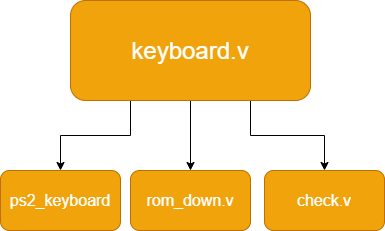
\includegraphics[width=1\textwidth]{kbd_struct.png}
  \caption{键盘部分的模块层次结构}
  \label{kbd_struct}
\end{figure}


\section{VGA部分}
VGA部分基本沿用前序实验内容。为了FPGA资源分配得当,
我们不得不缩小了显存的显示范围,从$30\times70$缩小到$15\times20$。
VGA部分只承担扫描位置的字符ASCII转为屏幕显示。

\section{内存模块}
所有的内存写入只能在内存模块\mbox{mem\_ram.v}进行。
除了基础的读写使能控制,我们还需要用assign连线
将VGA扫描到的值输出至屏幕上。此外,当回车键按下时
(由cmd\_flag判断),我们需要根据prog\_type的类型
输出对应的打印命令到屏幕上。

此外,我们会根据prog\_type信号把当前可能存在的参数存放到内存的数据区。
同时把对应程序的指令数PC\_end输出,提供给CPU模块。
在CPU执行汇编指令时,PC\_end会被用于判断程序的当前指令是否是最后一条指令。


\section{指令模块}
和内存模块一样,指令模块也是一个存储器所在的模块,
有着和其他存储器模块一样的通用接口。指令模块的功能是:
在读使能有效时,根据prog\_type的种类选择执行
对应的硬编码在内存中的指令。


\section{顶层模块}
在顶层模块中,我们为CPU提供了一段时长为5个周期的
缓冲时间,用信号init来进行控制。在经过这段时间后,
CPU就可以启动了:
\begin{lstlisting}[style=verilog-style]
reg [2:0] init, cnt;
parameter [2:0] set_time = 5;

initial begin
  init = 0;
  cnt = 0;
  mem_addr=0;
  cpu_en=0;
end

always @ (posedge clk) begin
  if (init < set_time) begin
    init <= init+1;
  end
end

always @ (posedge clk) begin
  if (init == set_time) begin
    if (enter_flag==1) begin
      cpu_en <= 1;
      cnt <= 0;
    end else if (cnt == set_time) begin
      if (cpu_finished==1) cpu_en <= 0;
    end else begin
      cnt <= cnt + 1;
    end
  end
end
\end{lstlisting}

在顶层模块中,我们会判断此时是CPU还是键盘在对内存写入。
主要由cpu\_en信号做选择控制:
\begin{lstlisting}[style=verilog-style]
always @ (*) begin
	if(cpu_en==1)begin
		mem_re=cpu_mem_re;
		mem_we=cpu_mem_we;
		mem_addr=cpu_mem_addr;
		mem_w_data=cpu_rt_data;
	end else begin
		mem_we=key_mem_we;
		mem_addr=key_mem_addr;
		mem_w_data=ascii;
	end
end
\end{lstlisting}


\section{测试方法}
在CPU模块编写完成之后,我们针对所有MIPS汇编指令
一共编写了4个测试文件,进行仿真。我们对每一条指令
分析时序、检查读写存储器的结果,确保CPU模块没有错误。

汇编指令测试文件:
\begin{itemize}
  \item alu\_R\_unsigned.txt
  \item alu\_R\_signed.txt
  \item alu\_I\_type.txt
  \item jp\_br\_mem.txt
\end{itemize}

\begin{figure}[H]
  \centering
  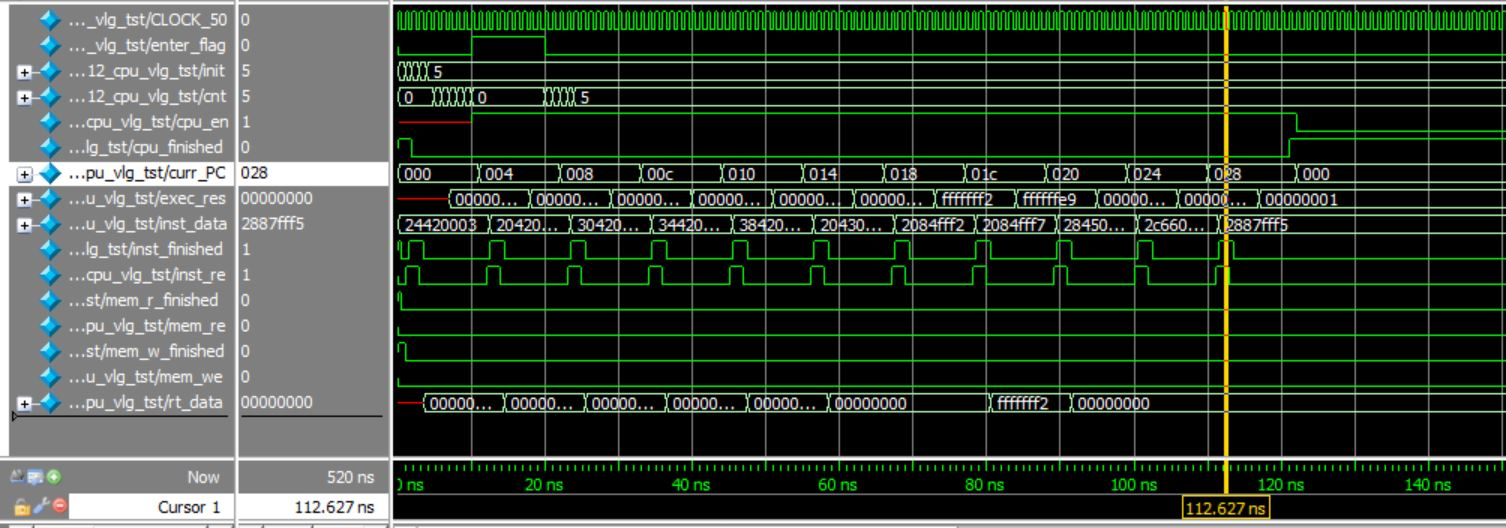
\includegraphics[width=1\textwidth]{sim_cpu.JPG}
  \caption{对CPU模块的仿真}
  \label{sim_cpu}
\end{figure}

将键盘模块与内存连接之后,也编写了测试文件进行仿真:
\begin{figure}[H]
  \centering
  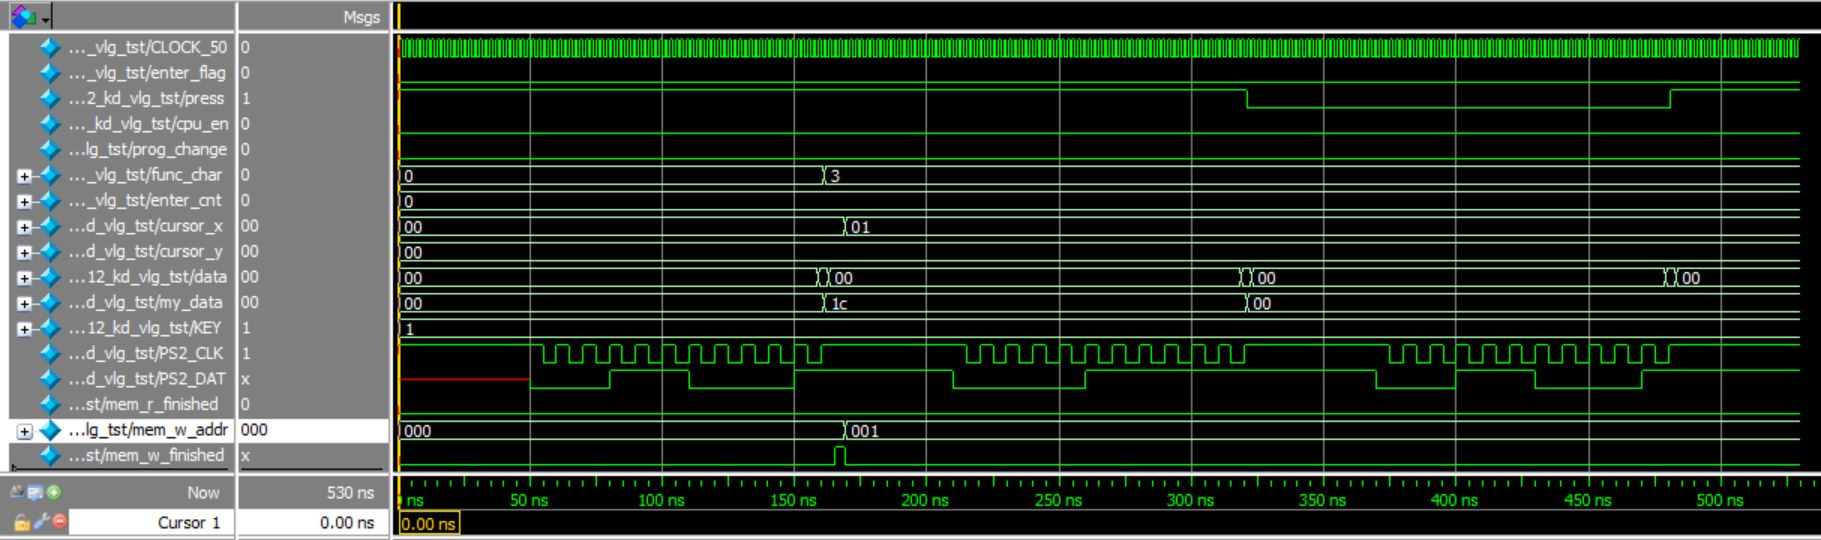
\includegraphics[width=1\textwidth]{sim_kd.JPG}
  \caption{对键盘模块的仿真}
  \label{sim_kd}
\end{figure}

然后将CPU、键盘、存储器都连接起来,对整个工程进行仿真:
\begin{figure}[H]
  \centering
  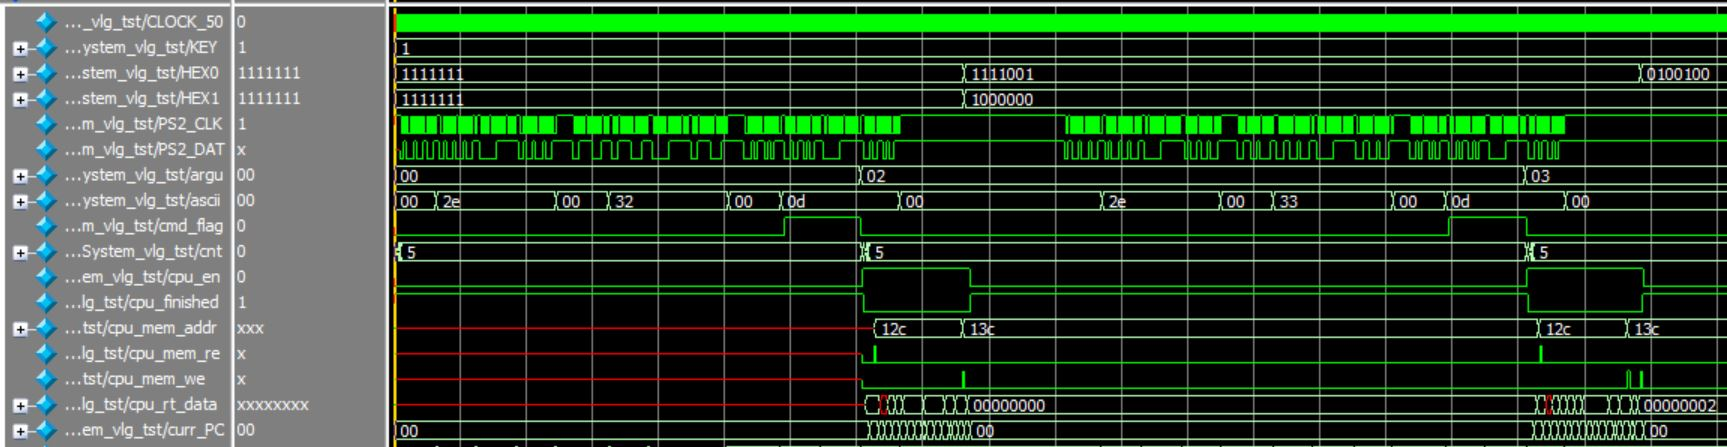
\includegraphics[width=1\textwidth]{sim_all.JPG}
  \caption{对整个工程的仿真}
  \label{sim_all}
\end{figure}


\section{实验结果}
\begin{figure}[H]
  \centering
  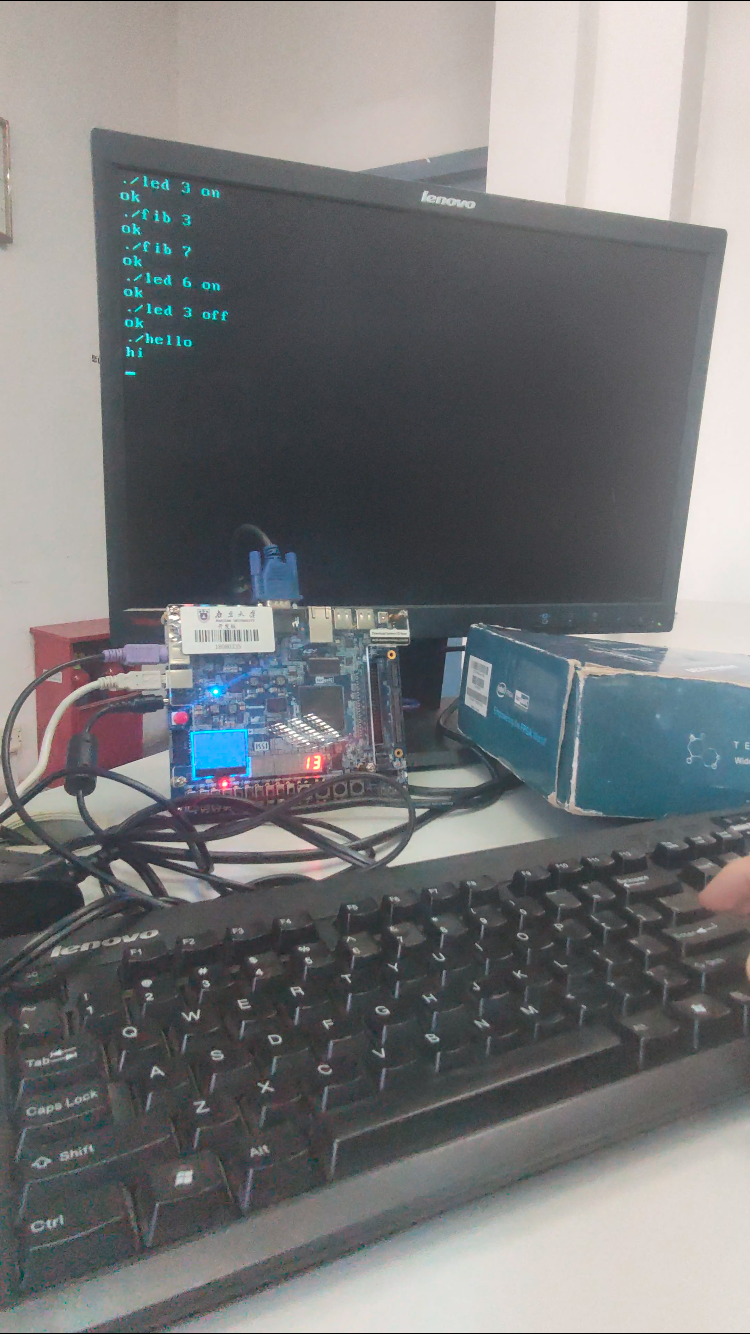
\includegraphics[width=0.7\textwidth]{fpga.PNG}
  \caption{下载运行}
  \label{fpga}
\end{figure}

\newpage

\part{问题总结}
\section{遇到的问题及解决办法}
\begin{itemize}
  \item 在分析CPU状态机时序的时候,发现cpu\_finished信号会产生抖动。
        对该信号的赋值语句稍作修改即可消抖。
  \item 刚开始构建CPU时,我们把指令存储器、寄存器文件、内存这三个存储器
        所属的模块都作为CPU模块的子模块了。后来发现许多其他的模块(如键盘、
        显示器等)都需要对指令和内存进行读写,如果这些读写都需要经过
        CPU模块才能访问到存储器,那么显然这么划分模块不太合适。所以
        我们最终决定在顶层模块中实例化指令存储器和内存存储器所属的模块。
        对于其他模块如CPU、键盘等,把它们需要读写的内容先输出到顶层模块中,
        然后再输入到存储器模块中进行读写。
  \item 仿真的时候,工程文件中不能包含缺少敏感信息列表的always块。否则
        仿真会一直卡在那里,不显示Wave波形且不报错。只有当关闭
        仿真程序时,它才会显示卡死的模块位置
  \item 字符串比较的思路是:把普通字符存入缓存buf,回车时取出全部buf内容,
        然后通过硬件的编码判断。但最开始时采用了CLOCK\_50这个高速的时钟频率,
        这导致按下一个键,buf的所有位置都会被写入同一个值。

        解决方法是将always块中的CLOCK\_50上升沿触发改成每次按键松开时触发,
        即PS2模块输入在遇到断码0xf0时进行一系列判断。但是这会分裂出一个
        不统一在CLOCK\_50内的逻辑语块。最后我们通过增加信号配合的方式,
        纠正衍生的时序错位。
  \item 键盘模块之间很容易产生错乱的时序问题,通常是由于时钟周期不一致
        导致了信号的衔接错误。相关的时钟主要包括键盘模块按键的时钟和
        VGA模块屏幕刷新的时钟。解决方法是都把这些时钟都回归到CLOCK\_50,
        用key\_off计数的方式维持原来的输入输出效果。
  \item 最令人头疼的是FPGA资源不足的问题。我们不得不进行很多删减,
        从而压缩尽可能多的内存开销,以保留核心功能。
\end{itemize}

\section{得到的启示}
\begin{itemize}
  \item 遇到bug时尽量用仿真进行debug。下载运行一个星期都没找到原因的bug,
        最后花了一下午做了个仿真,轻轻松松定位bug并分析出了原因。
  \item 存储器还是尽量用IP核。我们在设计CPU的时候没考虑过使用IP核,
        直接自己设计了存储器及其接口。这会导致一次编译要花大量的时间。
  \item 字符串比较和按键回显还是应该让CPU执行汇编指令来处理。用Verilog写
        会导致占用大量的FPGA资源,最后导致资源不够的问题。
\end{itemize}


\section{意见和建议}
我们发现这个实验最难的部分不是CPU部分,而是键盘输入、显示器输出、
以及它们对内存的读写这部分。我们用一个星期写完了CPU部分,用4个测试文件
测试CPU的30条汇编指令,一个bug都没有出。这导致我们放松了警惕,认为
键盘和显示器部分不过是复用前面几个实验的内容,不会太过困难。但事与愿违,
我们在这一块整整卡了大半个月的bug,才勉勉强强搞定。

所以对于题目提供的pdf文件,我们有这样的建议:CPU部分介绍得非常好,
它极为详细地为我们描述了实现CPU的方法,同时又最大程度上地
保证了实现方式的多样性,不会限制同学们的思路。输入输出部分可以
再多介绍一些。例如可以描述键盘和显示器如何读写内存、
如何用汇编指令实现按键回显等等。

我读完题目pdf之后最大的感受是,
这个实验所要实现的功能完全可以直接用Verilog代码来实现,
完全可以不用CPU执行汇编来实现软件功能。题目pdf可以多阐述一些
汇编可以实现的功能,并给出一两个汇编例子,比如删除键或回车键的例子。
这会引导同学们从汇编的角度思考如何处理按键回显,而不是像
前几个实验那样简单地用Verilog处理按键。

\end{document}